%%%%%%%%%%%%%%%%%%%%%%%%%%%%%%%%%%%%%%%%%
% Beamer Presentation
% LaTeX Template
% Version 1.0 (10/11/12)
%
% This template has been downloaded from:
% http://www.LaTeXTemplates.com
%
% License:
% CC BY-NC-SA 3.0 (http://creativecommons.org/licenses/by-nc-sa/3.0/)
%
%%%%%%%%%%%%%%%%%%%%%%%%%%%%%%%%%%%%%%%%%

%----------------------------------------------------------------------------------------
%	PACKAGES AND THEMES
%----------------------------------------------------------------------------------------

\documentclass{beamer}

\mode<presentation> {

% The Beamer class comes with a number of default slide themes
% which change the colors and layouts of slides. Below this is a list
% of all the themes, uncomment each in turn to see what they look like.

%\usetheme{default}
%\usetheme{AnnArbor}
%\usetheme{Antibes}
%\usetheme{Bergen}
%\usetheme{Berkeley}
%\usetheme{Berlin}
%\usetheme{Boadilla}
%\usetheme{CambridgeUS}
%\usetheme{Copenhagen}
%\usetheme{Darmstadt}
%\usetheme{Dresden}
%\usetheme{Frankfurt}
%\usetheme{Goettingen}
%\usetheme{Hannover}
%\usetheme{Ilmenau}
%\usetheme{JuanLesPins}
%\usetheme{Luebeck}
\usetheme{Madrid}
%\usetheme{Malmoe}
%\usetheme{Marburg}
%\usetheme{Montpellier}
%\usetheme{PaloAlto}
%\usetheme{Pittsburgh}
%\usetheme{Rochester}
%\usetheme{Singapore}
%\usetheme{Szeged}
%\usetheme{Warsaw}

% As well as themes, the Beamer class has a number of color themes
% for any slide theme. Uncomment each of these in turn to see how it
% changes the colors of your current slide theme.

%\usecolortheme{albatross}
%\usecolortheme{beaver}
%\usecolortheme{beetle}
%\usecolortheme{crane}
%\usecolortheme{dolphin}
%\usecolortheme{dove}
%\usecolortheme{fly}
%\usecolortheme{lily}
%\usecolortheme{orchid}
%\usecolortheme{rose}
%\usecolortheme{seagull}
%\usecolortheme{seahorse}
%\usecolortheme{whale}
%\usecolortheme{wolverine}

%\setbeamertemplate{footline} % To remove the footer line in all slides uncomment this line
%\setbeamertemplate{footline}[page number] % To replace the footer line in all slides with a simple slide count uncomment this line

%\setbeamertemplate{navigation symbols}{} % To remove the navigation symbols from the bottom of all slides uncomment this line
}

\usepackage{geometry}
\usepackage{multimedia}  % Allows including videos
\usepackage{graphicx}    % Allows including images
\usepackage{bm}          % Allows nice bold math
\usepackage{color}       % Allows color
\usepackage{array,booktabs,calc} % Allows nice multi-figure layout
\usepackage{setspace}

\definecolor{light_green}{rgb}{0.8,1.,0.8}
\definecolor{light_yellow}{rgb}{1.,1.,0.8}
\definecolor{yellow}{rgb}{1.,1.,0.}
\definecolor{orange}{rgb}{0.9,0.4,0.}
\definecolor{pink}{rgb}{1.,0.6,1.}
\definecolor{dark_green}{rgb}{0.1,0.6,0.1}
\definecolor{light_blue}{rgb}{0.6,0.6,1.}
\definecolor{purple}{rgb}{0.8,0.0,0.8}
\def\oran#1{\color{orange} #1}
\def\gr#1{\color{dark_green} #1}
\def\re#1{\color{red}   #1}
\def\bl#1{\color{blue}  #1}
\def\pu#1{\color{purple} #1}
\def\bk#1{\color{black} #1}
\def\lb#1{\color{light_blue} #1}
\def\pk#1{\color{pink} #1}
\def\ye#1{\color{yellow} #1}

\providecommand\der{{\rm d}}
\providecommand\Der{{\rm D}}
\providecommand\pa{{\partial}}
\def\pp#1#2{\frac{\pa  #1}{\pa  #2}}
\def\dd#1#2{\frac{\der #1}{\der #2}}
\def\DD#1#2{\frac{\Der #1}{\Der #2}}

\def\ltw{{\hbox{${\lower 6pt\hbox{$<$}}\atop{\raise 2pt\hbox{$\sim$}}$}\,}}
\def\gtw{{\hbox{${\lower 6pt\hbox{$>$}}\atop{\raise 2pt\hbox{$\sim$}}$}\,}}

\newcommand\shalf{\ensuremath{{\scriptstyle\frac{1}{2}}}}
\newcommand\sh{\ensuremath{^{\shalf}}}
\newcommand\sthalf{\ensuremath{{\scriptstyle\frac{3}{2}}}}
\newcommand\sth{\ensuremath{^{\sthalf}}}
\newcommand\smh{\ensuremath{^{-\shalf}}}
\newcommand\squart{\ensuremath{{\textstyle\frac{1}{4}}}}
\newcommand\thalf{\ensuremath{{\textstyle\frac{1}{2}}}}

\newcommand{\cO}{\ensuremath{\mathcal{O}}}
\newcommand{\cC}{\ensuremath{\mathcal{C}}}
\newcommand{\cD}{\ensuremath{\mathcal{D}}}
\newcommand{\cF}{\ensuremath{\mathcal{F}}}

\newcommand{\bel}{\ensuremath{b_\ell}}
\newcommand{\bli}{\ensuremath{b_{\ell i}}}
\newcommand{\blb}{\ensuremath{b_{\ell 0}}}
\newcommand{\thlo}{\ensuremath{\theta_{\ell 0}}}
\newcommand{\thpl}{\ensuremath{\theta'_{\ell}}}

\newsavebox{\AAbox} \sbox{\AAbox}{\boldmath$A$}
\newcommand{\Abf}{\usebox{\AAbox}}

\newsavebox{\SSbox} \sbox{\SSbox}{\boldmath$S$}
\newcommand{\Sbf}{\usebox{\SSbox}}

\newsavebox{\FFbox} \sbox{\FFbox}{\boldmath$F$}
\newcommand{\Fbf}{\usebox{\FFbox}}

\newsavebox{\GGbox} \sbox{\GGbox}{\boldmath$G$}
\newcommand{\Gbf}{\usebox{\GGbox}}

\newsavebox{\HHbox} \sbox{\HHbox}{\boldmath$H$}
\newcommand{\Hbf}{\usebox{\HHbox}}

\newsavebox{\eebox} \sbox{\eebox}{\boldmath$e$}
\newcommand{\ee}{\usebox{\eebox}}
\newcommand{\eex}{\ensuremath{\hat{\ee}_x}}
\newcommand{\eey}{\ensuremath{\hat{\ee}_y}}
\newcommand{\eez}{\ensuremath{\hat{\ee}_z}}

\newcommand{\bcdot}{\bm \cdot}
\newcommand{\oo}{\bm \omega}
\newcommand{\uu}{\bm u}
\newcommand{\xx}{\bm x}
\newcommand{\XX}{\bm X}

\newcommand{\grad}{\bm \nabla}
\newcommand{\degrees}{\mbox{$^{\circ}$}}

\let\vaccent=\v % rename builtin command \v{} to \vaccent{}
\renewcommand{\v}[1]{\ensuremath{\mathbf{#1}}} % for vectors
%\renewcommand{\v}[1]{\ensuremath{\mbox{\boldmath$ #1 $}}}
\newcommand{\gv}[1]{\ensuremath{\mbox{\boldmath$ #1 $}}}
% for vectors of Greek letters
\newcommand{\uv}[1]{\hat{\ensuremath{\mathbf{ #1 }}}} % for unit vector
\newcommand{\abs}[1]{\left| #1 \right|} % for absolute value
\newcommand{\avg}[1]{\left< #1 \right>} % for average
\let\underdot=\d % rename builtin command \d{} to \underdot{}
\renewcommand{\d}[2]{\frac{d #1}{d #2}} % for derivatives
\newcommand{\pd}[2]{\frac{\partial #1}{\partial #2}}
% for partial derivatives
\let\divsymb=\div % rename builtin command \div to \divsymb
\renewcommand{\div}[1]{\v{\nabla} \cdot #1} % for divergence
\newcommand{\curl}[1]{\v{\nabla} \times #1} % for curl

\usepackage{fancyvrb}
\DefineShortVerb[commandchars=\\\{\}]{\|}
\DefineVerbatimEnvironment{Highlighting}{Verbatim}{commandchars=\\\{\}}
% Add ',fontsize=\small' for more characters per line
\newenvironment{Shaded}{}{}
\newcommand{\KeywordTok}[1]{\textcolor[rgb]{0.13,0.29,0.53}{\textbf{{#1}}}}
\newcommand{\DataTypeTok}[1]{\textcolor[rgb]{0.13,0.29,0.53}{{#1}}}
\newcommand{\DecValTok}[1]{\textcolor[rgb]{0.00,0.00,0.81}{{#1}}}
\newcommand{\BaseNTok}[1]{\textcolor[rgb]{0.00,0.00,0.81}{{#1}}}
\newcommand{\FloatTok}[1]{\textcolor[rgb]{0.00,0.00,0.81}{{#1}}}
\newcommand{\ConstantTok}[1]{\textcolor[rgb]{0.00,0.00,0.00}{{#1}}}
\newcommand{\CharTok}[1]{\textcolor[rgb]{0.31,0.60,0.02}{{#1}}}
\newcommand{\SpecialCharTok}[1]{\textcolor[rgb]{0.00,0.00,0.00}{{#1}}}
\newcommand{\StringTok}[1]{\textcolor[rgb]{0.31,0.60,0.02}{{#1}}}
\newcommand{\VerbatimStringTok}[1]{\textcolor[rgb]{0.31,0.60,0.02}{{#1}}}
\newcommand{\SpecialStringTok}[1]{\textcolor[rgb]{0.31,0.60,0.02}{{#1}}}
\newcommand{\ImportTok}[1]{{#1}}
\newcommand{\CommentTok}[1]{\textcolor[rgb]{0.56,0.35,0.01}{\textit{{#1}}}}
\newcommand{\DocumentationTok}[1]{\textcolor[rgb]{0.56,0.35,0.01}{\textbf{\textit{{#1}}}}}
\newcommand{\AnnotationTok}[1]{\textcolor[rgb]{0.56,0.35,0.01}{\textbf{\textit{{#1}}}}}
\newcommand{\CommentVarTok}[1]{\textcolor[rgb]{0.56,0.35,0.01}{\textbf{\textit{{#1}}}}}
\newcommand{\OtherTok}[1]{\textcolor[rgb]{0.56,0.35,0.01}{{#1}}}
\newcommand{\FunctionTok}[1]{\textcolor[rgb]{0.00,0.00,0.00}{{#1}}}
\newcommand{\VariableTok}[1]{\textcolor[rgb]{0.00,0.00,0.00}{{#1}}}
\newcommand{\ControlFlowTok}[1]{\textcolor[rgb]{0.13,0.29,0.53}{\textbf{{#1}}}}
\newcommand{\OperatorTok}[1]{\textcolor[rgb]{0.81,0.36,0.00}{\textbf{{#1}}}}
\newcommand{\BuiltInTok}[1]{{#1}}
\newcommand{\ExtensionTok}[1]{{#1}}
\newcommand{\PreprocessorTok}[1]{\textcolor[rgb]{0.56,0.35,0.01}{\textit{{#1}}}}
\newcommand{\AttributeTok}[1]{\textcolor[rgb]{0.77,0.63,0.00}{{#1}}}
\newcommand{\RegionMarkerTok}[1]{{#1}}
\newcommand{\InformationTok}[1]{\textcolor[rgb]{0.56,0.35,0.01}{\textbf{\textit{{#1}}}}}
\newcommand{\WarningTok}[1]{\textcolor[rgb]{0.56,0.35,0.01}{\textbf{\textit{{#1}}}}}
\newcommand{\AlertTok}[1]{\textcolor[rgb]{0.94,0.16,0.16}{{#1}}}
\newcommand{\ErrorTok}[1]{\textcolor[rgb]{0.64,0.00,0.00}{\textbf{{#1}}}}
\newcommand{\NormalTok}[1]{{#1}}
%~ \ifxetex
  %~ \usepackage[setpagesize=false, % page size defined by xetex
              %~ unicode=false, % unicode breaks when used with xetex
              %~ xetex,
              %~ colorlinks=true,
              %~ linkcolor=blue]{hyperref}
%~ \else
  %~ \usepackage[unicode=true,
              %~ colorlinks=true,
              %~ linkcolor=blue]{hyperref}
%~ \fi
\hypersetup{breaklinks=true, pdfborder={0 0 0}}
\setlength{\parindent}{0pt}
\setlength{\parskip}{6pt plus 2pt minus 1pt}
\setlength{\emergencystretch}{3em}  % prevent overfull lines
\setcounter{secnumdepth}{0}

%\EndDefineVerbatimEnvironment{Highlighting}

\newcolumntype{C}[1]{>{\centering\arraybackslash}m{#1}}
\providecommand{\tightlist}{%
  \setlength{\itemsep}{0pt}\setlength{\parskip}{0pt}}

%----------------------------------------------------------------------------------------
%	TITLE PAGE
%----------------------------------------------------------------------------------------
%\title[LES discussions]{LES and more...}

\title[MPIC]{Webinar: Parallel Moist Parcel-In-Cell code}

\author[B\"oing, Gibb, Dritschel, et al.]{{Steef B\"oing, Gordon Gibb, David Dritschel, Nick Brown, \newline Mich\`ele Weiland, Doug Parker \& Alan Blyth}\vspace{-0.5cm}}

\institute[]{{University of Leeds, University of St Andrews, EPCC}\vspace{-0.4cm}}

\date{November 13, 2019}

\begin{document}

\begin{frame}

\titlepage % Print the title page as the first slide

\vspace{-0.6cm}
\begin{center}
%  \includegraphics[width = \textwidth]{pmpic_images/vorpic-cropped.pdf}
  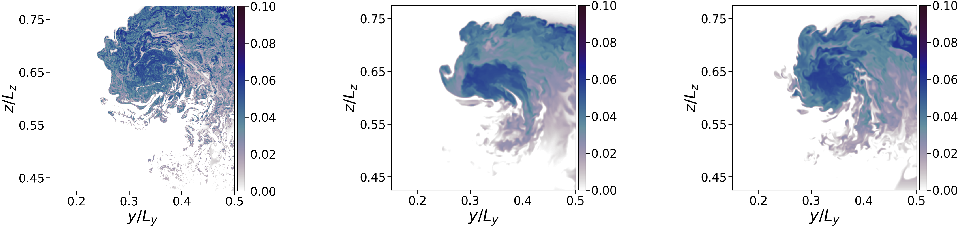
\includegraphics[width = \textwidth]{pmpic_images/croppedfig_les.pdf}
\end{center}

\setstretch{0.3} 

\end{frame}

\begin{frame}

\tableofcontents
\end{frame}

\begin{frame}
\frametitle{eCSE project 12-10}
\textit{A fully Lagrangian dynamical core for the Met Office NERC Cloud Model}
\vspace{-0.2cm}
\begin{center}
St Andrews, Leeds, EPCC
\end{center}
\vspace{-0.2cm}
\begin{itemize}
\item Most fluid dynamics codes are either fully Eulerian (grid-based), or semi-Lagrangian (advection using \textit{departure points} and regridding)
\item MPIC: \textit{essentially Lagrangian} (prognostics on parcels, solver uses grid)
\item Atmospheric Large-Eddy Simulation: e.g. Met Office NERC Cloud model. 
\item Evaporation and condensation in clouds: discontinuity in underlying equations.
\end{itemize}
\vspace{-0.8cm}

\begin{center}
  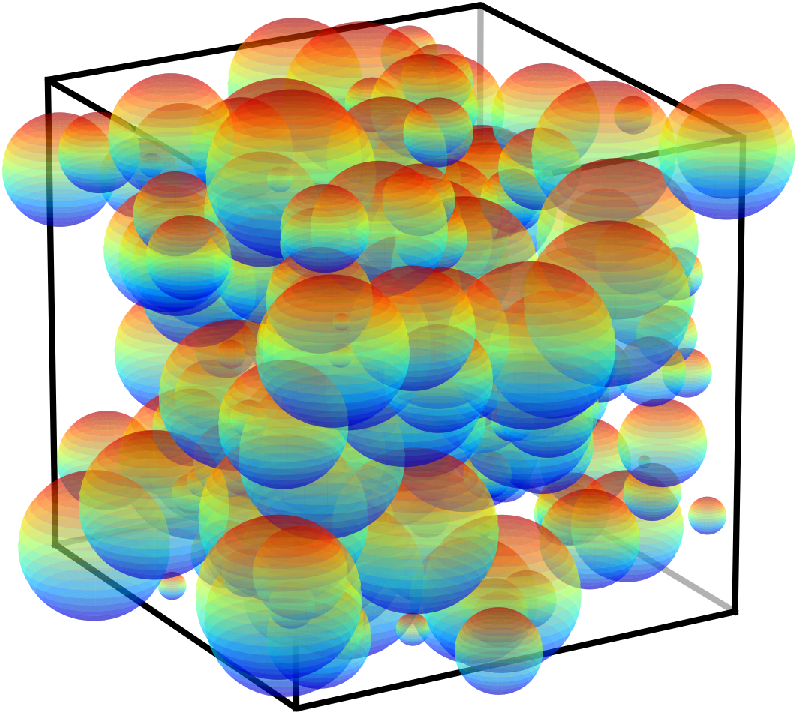
\includegraphics[width = 0.28\textwidth]{pmpic_images/parcels.pdf}
\end{center}

\end{frame}

\section{Moist Parcel-in-Cell code: overview}

%------------------------------------------------
\begin{frame}
\frametitle{Essentially Lagrangian modelling}

\begin{block}{}
{\bl The basic conservation principles} of fluid dynamics 
{\gr are naturally expressed} in a {\pu Lagrangian} way: 
e.g.\ mass is conserved {\it \re following} fluid ``parcels''.
\end{block}

\vspace{0.5cm}
{\re However}, certain fields are more naturally Eulerian in character,
e.g.\ pressure.  Here, one needs to solve for the entire field through
``inversion''.

\vspace{0.3cm}
\begin{block}{}
{\gr Conservation is Lagrangian.}  {\pu Inversion is Eulerian.}  
\end{block}

\vspace{0.5cm}
{\it Can we exploit this for simulation?}

\end{frame}

%-------------------------------------------------------------------

\begin{frame}
\frametitle{Moist Parcel-In-Cell (MPIC)}

The new ``Moist Parcel-In-Cell'' (MPIC) algorithm 
{\re represents the continuum by discrete} {\bl ``cloud (or environment) parcels''}.

\vspace{0.15cm}
We use {\pu freely-moving} 
{\pu parcels} carrying {\it any number} of {\re attributes} 
(e.g.\ {\bl a conserved temperature} 
$b_\ell$, {\bl specific humidity} $q$, etc...)

\vspace{0.15cm}
Prototype model for 3D incompressible flow
(Boussinesq, no rotation, no precipitation):
\begin{flalign}
\DD{\uu}{t} & = - \frac{\grad{p}}{\rho_0} + b \uv{z} \qquad & \textsf{momentum} \nonumber \\ 
\DD{\bel}{t}&  = 0  \qquad & \textsf{conserved temperature} \nonumber \\
\DD{q}{t} & = 0  \qquad & \textsf{specific humidity, total amount of water} \nonumber \\
\grad\bcdot\uu & =0  \qquad & \textsf{incompressibility} \nonumber  \\
\nonumber
\end{flalign}

\end{frame}

\begin{frame}
\frametitle{Phase transitions}
The {\re total buoyancy} $b$ is approximated by
\begin{equation}
b = \bel+\alpha q_\ell \,,\qquad q_\ell =q-q_s(z) \qquad \textsf{if } q>q_s(z) \textsf{, otherwise 0}.
\nonumber
\end{equation}

$q_\ell$ is the {\bl liquid water content}. \newline
$q_s$ is the {\oran saturation humidity}, which decreases with height. \newline
$\alpha$ is a scale factor related to the {\re latent heat of condensation.} \newline

\end{frame}

\begin{frame}
\frametitle{Solution}

Rather than evolving momentum, we evolve the vorticity:
\begin{equation}
  \pd{\gv{\omega}}{t} = ( \div{\v{F}},\div{\v{G}},\div{\v{H}}), \nonumber
\end{equation}
Where $\v{F} = \gv{\omega}u + b \uv{y} $, $\v{G}=\gv{\omega}v - b \uv{x}$, $\v{H}=\gv{\omega}w$ and $\v{u}= (u,v,w)$.

\vspace{0.5cm}

Vector Poisson solver (finite difference) to find velocity potential $\v{A}$ and velocity $\v{u} = - \curl{\v{A}}$.

\begin{equation}
  \gv{\omega} = \v{\nabla}^2 \v{A}. \nonumber
\end{equation}

Some further subtleties in ensuring the vorticity is divergence free.

\end{frame}

\begin{frame}
\frametitle{Parcel splitting and mixing}

\begin{itemize}
\item Parcels stretch and can split into 2 smaller parcels, depending on vorticity.
\item Splitting: creates new parcel. Old and new parcel are change position.
\item When parcel becomes too small: merged into surrounding parcels using conservative operation via grid.
\end{itemize}

\end{frame}

\begin{frame}
\frametitle{Elements of parallelism}

\begin{itemize}
\item Change of parcel position: advection, splitting (local)
\item Parcel merging (local)
\item Vector Poisson solver (global)
\end{itemize}

\end{frame}

\section{The Met Office NERC Cloud model (parallelisation framework)}

%-------------------------------------------------------------------
\begin{frame}
\frametitle{eCSE project}
\textit{A fully Lagrangian dynamical core for the Met Office NERC Cloud Model}
\vspace{0.2cm}
\begin{center}
St Andrews, Leeds, EPCC (Mich\`ele Weiland, Nick Brown, Gordon Gibb)
\end{center}

\vspace{0.1cm}
Ideas:
\begin{itemize}
\item Harness {\gr MONC's parallelism}: hybrid OpenMP+MPI.
\item Poisson solver available.
\item Approach: {\bl domain decomposition}, number of parcels per subdomain will vary (simplicity versus optimal load balancing).
\item {\re Lagrangian diagnostics} can feed back into standard MONC.
\item {\pu Component testing} using simplified code.
\end{itemize}

\end{frame}

\begin{frame}
\frametitle{Parallelism}

\vspace{0.2cm}
\begin{itemize}
\item Vector Poisson solver: requires global communication. {\bl Efficient algorithms} exist.
\item First implementation OpenMP. Inherent limitation of problem size. HPC trend to {\pu large distributed memory systems}. 
\item Much more {\re parcel data} than {\gr grid data}.
\item Parcel data: {\oran local communication}.
\end{itemize}

\centering

\end{frame}

\begin{frame}
\frametitle{PMPIC}
\begin{itemize}
\item Implementation of MPIC in MONC's framework.
\item Based on stripped version of MONC core.
\item Not compatible with other MONC components (parcels in model state, RK4 time step, different equations, non-staggered grid).
\item But uses (FFTs, grids) and extends (parcel parallelism) MONC infrastructure.
\item GIT repository + makefile.
\end{itemize}
\end{frame}

\section{Design and performance}

\begin{frame}
\frametitle{Design choices}
\begin{itemize}
\item Data held in arrays, rather than parcel-types (more difficult halo-swap, but efficient). \\
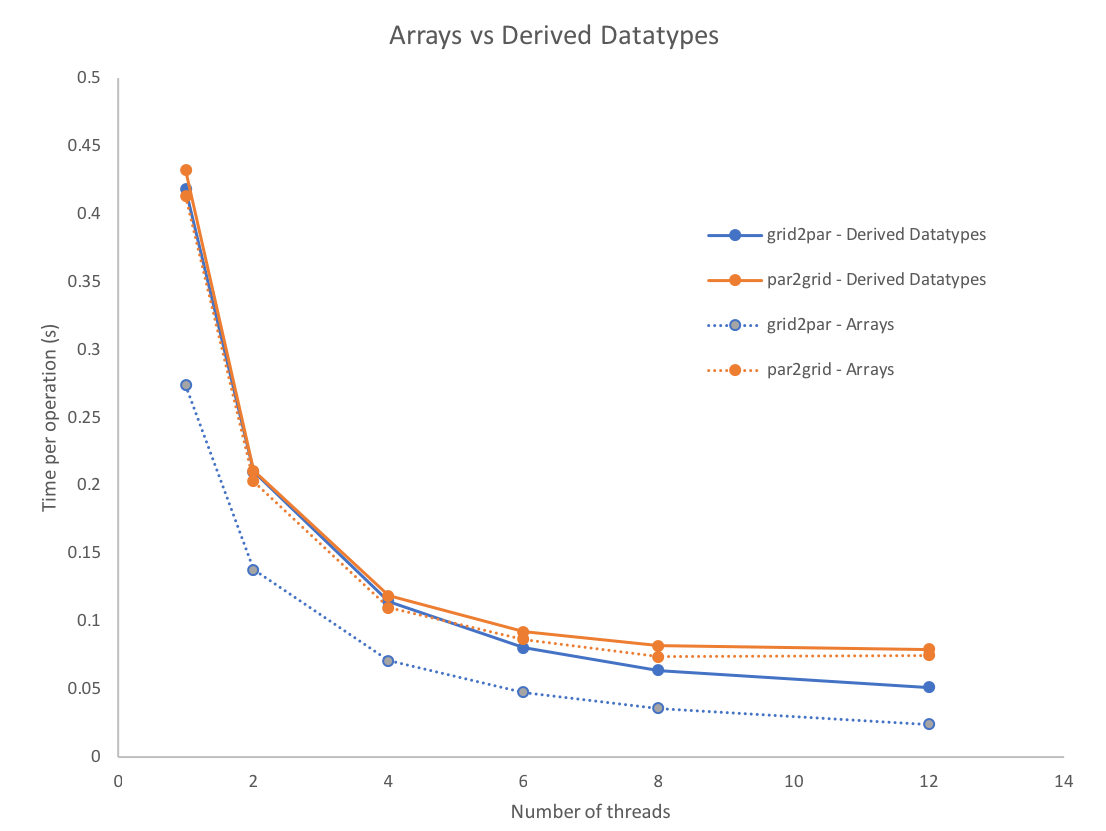
\includegraphics[width=0.45\textwidth]{pmpic_images/grid2par.png} 
\item New group type: RK4 (not all operations substepped). Note: higher memory footprint.
\item Binary dumps (parcels/grids) and NetCDF (optional, grids only so far), instead of IO-server. Memory requirements of main code.
\end{itemize}

\end{frame}

\begin{frame}
\frametitle{Halo-swapping}
\begin{itemize}
\item Parcel halo-swap needed testing. In particular: backfill.
\item Modified grid halo-swap in solver. Decision to write new simple halo-swapper for grids. 
\item Halo-swapping also comes into parcel mixing. Systematic parcel creation/removal tests.
\end{itemize}

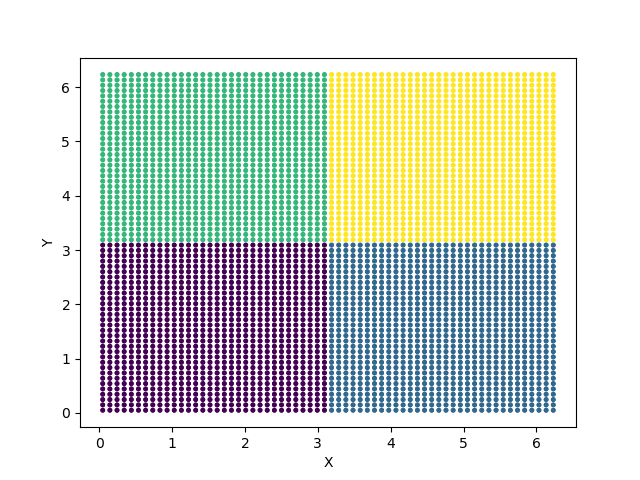
\includegraphics[width=0.45\textwidth]{pmpic_images/vel0.png} 
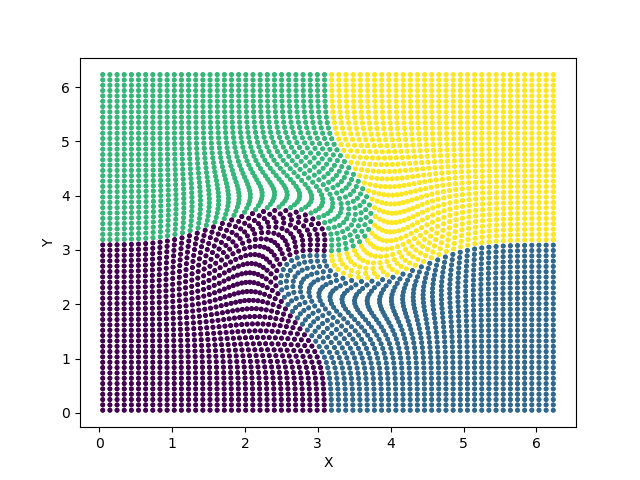
\includegraphics[width=0.45\textwidth]{pmpic_images/vel1.png} 

\end{frame}

\begin{frame}
\frametitle{Numerics}
\begin{itemize}
\item 4th order compact central differencing in tridiagonal solver (David Dritschel).
\end{itemize}

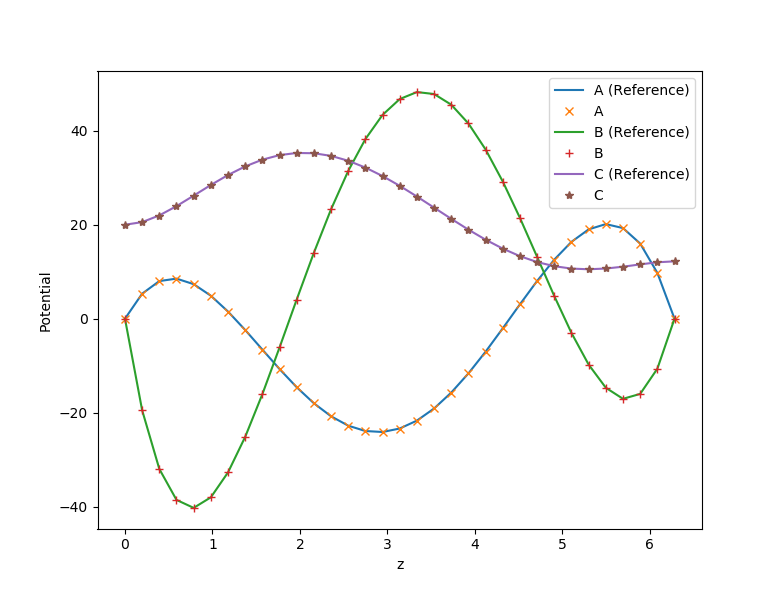
\includegraphics[width=0.70\textwidth]{pmpic_images/solution.png} 

\end{frame}

\begin{frame}
\frametitle{Performance: single node}

\begin{itemize}
\item Overall performance of new code on single core: 1.6 times faster.
\item MPI scaling hindred by load imbalance.
\item OpenMP not scaling well (might need to tune chunk size/refactor).
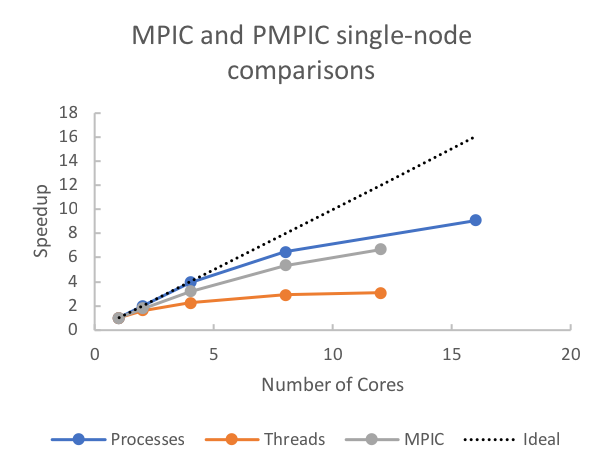
\includegraphics[width=0.45\textwidth]{pmpic_images/singleNode.png} 
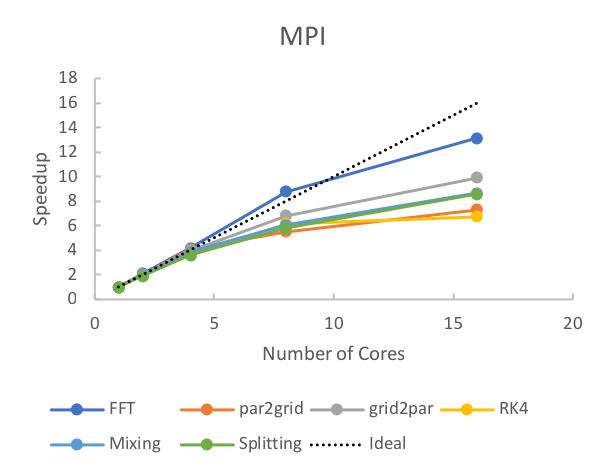
\includegraphics[width=0.45\textwidth]{pmpic_images/MPISingle.png} 
\end{itemize}

\end{frame}

\begin{frame}
\frametitle{Performance}

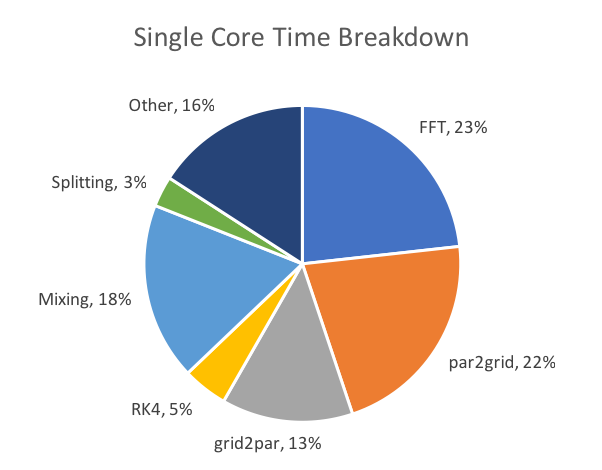
\includegraphics[width=0.90\textwidth]{pmpic_images/pie.png} 

\end{frame}

\begin{frame}
\frametitle{Performance: large simulations}

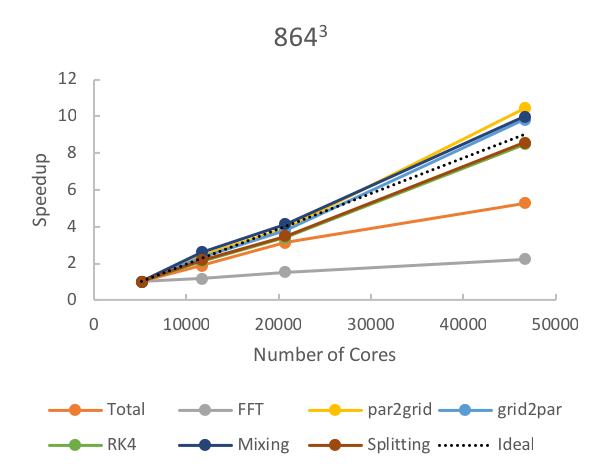
\includegraphics[width=0.45\textwidth]{pmpic_images/864.png} 
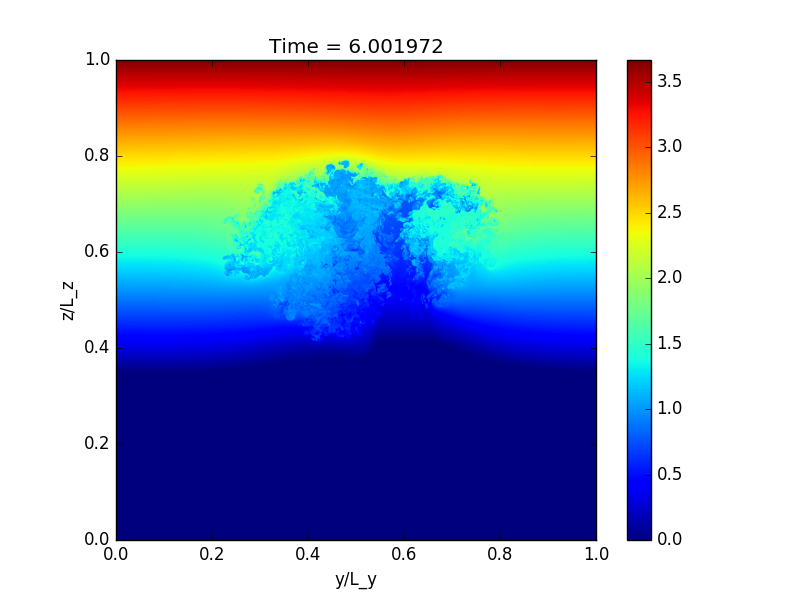
\includegraphics[width=0.45\textwidth]{pmpic_images/6.png} 

\end{frame}


\begin{frame}
\frametitle{Benefits}

\begin{itemize}
\item First use of this type of model in atmospheric community.
\item Massively parallel MPIC will make it more attractive for {\pu other problems}, e.g. ocean mixed layer, density-laden flows.
\item {\bl Alternative approach} for MONC community.
\item Could provide basis for Lagrangian diagnostics, currently {\re lacking in MONC}.
\item {\gr BSD} license.
\end{itemize}

\end{frame}

\hypertarget{welcome-to-the-pmpic-wiki}{%
\section{Repository, installation, adding components}\label{welcome-to-the-pmpic-wiki}}

\begin{frame}{PMPIC code repository}
\protect\hypertarget{pmpic-code-repository}{}

Example usage:

mpiexec -n 2 monc --config=config.mcf

Dependencies:

\begin{itemize}
\tightlist
\item
  MPI
\item
  FFTW
\end{itemize}

Compilers tested:

\begin{itemize}
\tightlist
\item
  GNU (on laptop and ARCHER)
\item
  Cray (on ARCHER)
\end{itemize}

Notes on compilation:

\begin{itemize}
\tightlist
\item
  See wiki page on this site
\end{itemize}

This code simulates the development of a plume using a Parcel-in-Cell
approach. A detailed technical description is given by Dritschel et al
2018 (QJRMS,
https://rmets.onlinelibrary.wiley.com/doi/abs/10.1002/qj.3319).

The code is currently constructed so that it uses as simple a set of
equations as possible. The default test case is a spherical moist and
warm thermal in a neutrally-stable boundary layer overlaid with a
stably-stratified atmosphere. The code is currently non-dimensional, and
uses idealised environmental profiles for stratification and
environmental humidity. It is also a tool for demonstrating the Parcel
in Cell method in a meteorological context, and shows how intricate
representations of cloud properties can be efficiently produced using
the method.

Mass, specific humidity and liquid-water potential temperature are
conserved following the motion of each parcel. Parcel vorticity is
evolved in the dynamical equations. MPIC has the advantages that it has
an explicit sub-grid representation and numerical dissipation is minimal
and can be controlled. The number of tuning parameters is kept to a
minimum.

Effects of latent heating are included by increasing the effective
buoyancy whenever the parcel specific humudity exceeds the
height-dependent saturation profile.

Mixing is included in the form of parcel splitting and merging.

The code is written in Fortran, and has been parallelised within the
eCSE project ``A fully Lagrangian dynamical core for the Met Office NERC
Cloud Model''

\end{frame}

\begin{frame}{Physics in PMPIC}
\protect\hypertarget{physics-in-pmpic}{}

The MPIC model is described
\href{https://rmets.onlinelibrary.wiley.com/doi/10.1002/qj.3319}{here}
and compared to MONC
\href{https://rmets.onlinelibrary.wiley.com/doi/abs/10.1002/qj.3532}{here}.

\end{frame}

\begin{frame}{PMPIC development}
\protect\hypertarget{pmpic-development}{}

Parallel MPIC was developed as part of eCSE project 12-10 ``A fully
Lagrangian dynamical core for the Met Office NERC Cloud Model''

\end{frame}

\begin{frame}[fragile]{Running PMPIC}
\protect\hypertarget{running-pmpic}{}

Running pmpic should be as simple as executing:

\texttt{{[}mpiexec/aprun\ ...{]}\ /path/to/monc\ -\/-config={[}config\ file{]}}

The config file controls which components are run (and in what order)
and also runtime parameters. There is also a global\_config file which
contains basic settings required for MONC to operate. This shouldn't be
edited unless you know what you're doing.

The config file and global\_config should be placed in the working
directory.

The default settings should run a 32\^{}3 gridcell simulation of a
spherical plume of moist buoyant air for 8 time units. When run on N
processes, it should produce 9N \texttt{grids\_*.dat} and
\texttt{parcels\_*.dat} files, n per process per time step.

The final files should have timestep number 144, and using
\texttt{display\_parcels.py} as

\texttt{python\ display\ parcels.py\ 144\ {[}N{]}}

(where N is the number of processes used in the simulation) you should
get the following image:

%\includegraphics{https://user-images.githubusercontent.com/17198605/49156538-82419900-f315-11e8-89a3-8533f580acc8.png}

Congratulations you have successfully run PMPIC!

The default case is small and should be able to run on a laptop in
around a minute or less.

\end{frame}

\begin{frame}[fragile]{Important}
\protect\hypertarget{important}{}

When the code is slow, please first try running with

\begin{Shaded}
\begin{Highlighting}[]
\BuiltInTok{export} \VariableTok{OMP_NUM_THREADS=}\NormalTok{1}
\end{Highlighting}
\end{Shaded}

as by default OpenMP uses all cores on your system, so you may end out
running many more threads+processes than you have cores.

\end{frame}

\begin{frame}{Components}
\protect\hypertarget{components}{}

==\textgreater{} basic\_parcelsetup/src/basic\_parcelsetup.F90
\textless{}==\\
!basic parcel setup - parcels are created to fill the volume with
n\_per\_dir parcels per\\
!grid cell per direction. Only x, y and z and vol.~All the other
properties are zero

==\textgreater{} debugger/src/debugger.F90 \textless{}==\\
!\textgreater{} General purpose debugger. By changing the priority and
other logic we can plug it in\\
!! whereever we want in the run to dump out information

==\textgreater{} decomposition/src/decomposition.F90 \textless{}==\\
!\textgreater{} Parallel decomposition to determine the grid points and
data columns that\\
!! are located on this process.

==\textgreater{} euler\_integrator/src/euler\_integrator.F90
\textless{}==\\
!A basic Euler integrator component (superseded by the RK4 integrator
component)

==\textgreater{} grid2partest/src/grid2partest.F90 \textless{}==\\
!sets up some parcels and grids then tests grid2par

==\textgreater{} haloswapper/src/haloswapper.F90 \textless{}==\\
!\textgreater{} Performs halo swapping. In the parallel case this is
between neighbouring processes\\
!! and in the serial case it still needs to wrap the halos around for
the boundary conditions. \textbf{(Not used) }

==\textgreater{} laplinv\_test/src/laplinv.F90 \textless{}==\\
!component that tests the tridiagonal laplacian inversion method

==\textgreater{} modelsynopsis/src/modelsynopsis.F90 \textless{}==\\
!\textgreater{} Displays information about the current state\_mod of the
model run

==\textgreater{} parcel\_mixing/src/parcel\_mixing.F90 \textless{}==\\
! Allows for parcel mixing - both the absorbtion and removal of small
parcels and adding in new parcels to fill holes

==\textgreater{} parcel\_splitting/src/parcel\_splitting.F90
\textless{}==\\
! This module splits parcels if they have obtained a stretch larger than
4\\
module parcel\_splitting\_mod

==\textgreater{} parcelsetup\_base/src/parcelsetup\_base.F90
\textless{}==\\
!reads in parcel options from config file and allocates memory. !Also
initialises parcel haloswapping and parcel interpolation routines. !
Does \textbf{not} place any parcels, merely allocate memory for them. !
This has to be done by a user-written component.

==\textgreater{} plume\_parcelsetup/src/plume\_parcelsetup.F90
\textless{}==\\
!Creates an initial condition of a spherical thermal from Dritschel et
al.~2018

==\textgreater{} prescribed\_parcel\_velocity/src/velocity.F90
\textless{}==\\
!Component that prescribes parcel velocities according to an analytical
velocity field !(test component - do not use on prodiction runs)

==\textgreater{}
readfromfile\_parcelsetup/src/readfromfile\_parcelsetup.F90
\textless{}==\\
!Recovers the model state from a saved parcel dump

==\textgreater{} rk4\_integrator/src/rk4\_integrator.F90 \textless{}==\\
!Runge Kutta 4th order integrator component

==\textgreater{} setup\_grid/src/setup\_grid.F90 \textless{}==\\
!Component to set up prognostic grids for Moist Parcel In Cell code\\
!This should be called before the parcelsetup component

==\textgreater{} simplesetup/src/simplesetup.F90 \textless{}==\\
! Sets up the thermal case (Not used)

==\textgreater{} terminationcheck/src/terminationcheck.F90 \textless{}==
!\textgreater{} This component will check for termination conditions at
stages of the model run and terminate that

==\textgreater{} vort2vel/src/vort2vel.F90 \textless{}==\\
!component that obtains the velocity from the vorticity via\\
! laplacian(A) = vort, where velocity = -curl(A)

==\textgreater{} vorticity\_tendency/src/vorticity\_tendency.F90
\textless{}==\\
!component that determines the vorticity tendency

==\textgreater{} writeparcels/src/writeparcels.F90 \textless{}==\\
!very basic parcel and grid writing routine

==\textgreater{} writegrids/src/writegrids.F90 \textless{}==\\
!netcdf grid writing routines

\end{frame}

\begin{frame}{Included scripts}
\protect\hypertarget{included-scripts}{}

display\_grid.py: displays a field (currently buoyancy)\\
display\_parcels.py: renders a field based on a Gaussian kernel\\
planner.py: calculates the approximate memory footprint of PMPIC (total
and per process)\\
timing.py: reads previously created timing data (need to specify this
beforehand in MONC configuration file)\\
visualise.py: older visualisation routine (obsolete?)

\end{frame}

\begin{frame}[fragile]{Writing your own initial condition component}
\protect\hypertarget{writing-your-own-initial-condition-component}{}

PMPIC comes with two initial condition components. The
\texttt{basic\_parcelsetup} component (which places parcels uniformly in
space but does not assign any values to them) and the
\texttt{plume\_parcelsetup} component which sets up the initial
condition used
\href{https://rmets.onlinelibrary.wiley.com/doi/10.1002/qj.3319}{here}.

To write your own initial condition component, it is easiest to create a
copy of the \texttt{basic\_parcelsetup} directory in
\texttt{components/} and call it something else (let's say
\texttt{my\_parcelsetup}). Change into this directory and alter the name
of \texttt{src/basic\_parcelsetup.F90} to
\texttt{src/my\_parcelsetup.F90}. Also remember to modify the makefile
in this directory to point to the newly renamed file.

Now to edit \texttt{my\_parcelsetup.F90}. First of all, change the
module name to \texttt{my\_parcelsetup\_mod}. Change the
\texttt{basic\_parcelsetup\_get\_descriptor} function to

\begin{Shaded}
\begin{Highlighting}[]
\DataTypeTok{type(component_descriptor_type)} \KeywordTok{function}\NormalTok{ my_parcelsetup_get_descriptor()}
\NormalTok{    my_parcelsetup_get_descriptor%name}\KeywordTok{=}\StringTok{"my_parcelsetup"}
\NormalTok{    my_parcelsetup_get_descriptor%version}\KeywordTok{=}\FloatTok{0.1}
\NormalTok{    my_parcelsetup_get_descriptor%initialisation}\KeywordTok{=}\OperatorTok{>}\NormalTok{initialisation_callback}

  \KeywordTok{end function}\NormalTok{ my_parcelsetup_get_descriptor}
\end{Highlighting}
\end{Shaded}

Now you can go and edit the subroutine \texttt{initalisation\_callback}
to put in the initial conditions you want.

To enable this component, alter your config file to have the line
\texttt{my\_parcelsetup\_enabled=.true.} (ensuring that the other
parcelsetup components are disabled).

After recompiling monc you should now be able to use your new component!

\end{frame}

\begin{frame}[fragile]{NetCDF libraries}
\protect\hypertarget{netcdf-libraries}{}

We have made output to Netcdf available in PMPIC. This requires a
version of netcdf with parallel netcdf support

These libraries are available under ARCHER as the cray-hdf5-parallel
cray-netcdf-hdf5parallel modules. Note that if you change compiler
environment (compilation has been tested with the GNU compiler on
ARCHER) you may need to unload and then reload the modules.

On your own system you may want to compile this version of netcdf as a
standalone version, in which case you will need to set the NETCDF\_ROOT
environment variable to the path where you compile it. This is a bit
tricky. Using ldd, you can check both which libraries monc is linked to
as well as how libraries (.so files) link to other libraries.

Compilation has been tested using the following libraries:

zlib-1.2.11 (https://zlib.net/)\\
hdf5-1.10.4
(https://support.hdfgroup.org/ftp/HDF5/prev-releases/hdf5-1.10/hdf5-1.10.4/src/)\\
netcdf-4.6.1 (https://www.unidata.ucar.edu/downloads/netcdf/index.jsp)\\
netcdf-fortran-4.4.4
(https://www.unidata.ucar.edu/downloads/netcdf/index.jsp)

For compilation, extract the tarballs, and make a directory to compile
the libraries (e.g. \$HOME/dependencies).

For zlib:

\begin{Shaded}
\begin{Highlighting}[]
\ExtensionTok{./configure}\NormalTok{ --prefix=}\VariableTok{\$HOME}\NormalTok{/dependencies/zlib CC=mpicc  }
\FunctionTok{sudo}\NormalTok{ make install}
\end{Highlighting}
\end{Shaded}

For HDF5

\begin{Shaded}
\begin{Highlighting}[]
\ExtensionTok{./configure}\NormalTok{ --with-zlib=}\VariableTok{$HOME}\NormalTok{/dependencies/zlib --enable-parallel \textbackslash{}}
\NormalTok{--prefix=}\VariableTok{$HOME}\NormalTok{/dependencies/hdf5 CC=mpicc CXX=mpicxx FC=mpif90  }
\FunctionTok{sudo}\NormalTok{ make install}
\end{Highlighting}
\end{Shaded}

In some cases. you may need to be even more specific (i.e.~provide the
full path) about the location of mpicc/mpicxx/mpif90. For netcdf (C,
with the CURL library disabled)

\begin{Shaded}
\begin{Highlighting}[]
\ExtensionTok{./configure}\NormalTok{ CPPFLAGS=\textbackslash{}}
\StringTok{"-I }\VariableTok{$HOME}\StringTok{/dependencies/zlib/include -I }\VariableTok{$HOME}\StringTok{/dependencies/hdf5/include"}\NormalTok{ \textbackslash{}}
\NormalTok{LDFLAGS=}\StringTok{"-L}\VariableTok{$HOME}\StringTok{/dependencies/hdf5/lib -L}\VariableTok{$HOME}\StringTok{/dependencies/zlib/lib"}\NormalTok{ \textbackslash{}}
\NormalTok{--prefix=}\VariableTok{$HOME}\NormalTok{/dependencies/netcdf CC=mpicc FC=mpif90 \textbackslash{}}
\NormalTok{--enable-netcdf4 --disable-dap  }
\FunctionTok{sudo}\NormalTok{ make install}
\end{Highlighting}
\end{Shaded}

For netcdf (FORTRAN, here installed in the same directory after NETCDF
C, note you will need both)

\begin{Shaded}
\begin{Highlighting}[]
\ExtensionTok{./configure}\NormalTok{ CPPFLAGS=\textbackslash{}}
\StringTok{"-I }\VariableTok{$HOME}\StringTok{/dependencies/zlib/include -I }\VariableTok{$HOME}\StringTok{/dependencies/hdf5/include -I }\VariableTok{$HOME}\StringTok{/dependencies/netcdf/include"}\NormalTok{ \textbackslash{}}
\NormalTok{LDFLAGS=}\StringTok{"-L}\VariableTok{$HOME}\StringTok{/dependencies/hdf5/lib -L}\VariableTok{$HOME}\StringTok{/dependencies/netcdf/lib -L}\VariableTok{$HOME}\StringTok{/dependencies/netcdf/lib"}\NormalTok{ \textbackslash{}}
\NormalTok{--prefix=}\VariableTok{$HOME}\NormalTok{/dependencies/netcdf CC=mpicc FC=mpif90}
\FunctionTok{sudo}\NormalTok{ make install}
\end{Highlighting}
\end{Shaded}

The compilation settings can be found by running:

\begin{Shaded}
\begin{Highlighting}[]
\VariableTok{\$HOME}\ExtensionTok{/dependencies/netcdf/bin/nf-config}\NormalTok{ --all}
\end{Highlighting}
\end{Shaded}

Finally, you may need to set:

\begin{Shaded}
\begin{Highlighting}[]
\BuiltInTok{export} \VariableTok{LD_LIBRARY_PATH=}\StringTok{"}\VariableTok{$HOME}\StringTok{/dependencies/netcdf/lib:}\VariableTok{\$HOME}\StringTok{/dependencies/hdf5/lib:}\VariableTok{\$HOME}\StringTok{/dependencies/zlib/lib:}\VariableTok{$LD_LIBRARY_PATH}\StringTok{"}
\end{Highlighting}
\end{Shaded}

and

\begin{Shaded}
\begin{Highlighting}[]
\BuiltInTok{export} \VariableTok{NETCDF_ROOT=}\StringTok{"}\VariableTok{\$HOME}\StringTok{/dependencies/netcdf/"}
\end{Highlighting}
\end{Shaded}

and

\begin{Shaded}
\begin{Highlighting}[]
\BuiltInTok{export} \VariableTok{PKG_CONFIG_PATH=}\StringTok{"}\VariableTok{\$HOME}\StringTok{/dependencies/netcdf/lib/pkgconfig/:}\VariableTok{\$PKG_CONFIG_PATH}\StringTok{"}
\end{Highlighting}
\end{Shaded}

Before running. It could be worth adding these to your .bashrc file.
Note, however, that setting the LD\_LIBRARY\_PATH may cause ncview to
generate an error. You may want to set

\begin{Shaded}
\begin{Highlighting}[]
\BuiltInTok{export} \VariableTok{HDF5_DISABLE_VERSION_CHECK=}\NormalTok{1}
\end{Highlighting}
\end{Shaded}

Or empty the LD\_LIBRARY\_PATH before using ncview.

\end{frame}

\section{Conclusions and future work}

\begin{frame}
\frametitle{Conclusions and future work}

\begin{itemize}
\item eCSE outcome: MPIC model that scales on thousands of cores.
\item Improving scalability: analyse issues with OpenMP, replace FFT-derivatives by compact finite difference (currently 18 FFTs per time step).  
\end{itemize}

\end{frame}

%-------------------------------------------------------------------

\begin{frame}
\frametitle{Further steps}

\vspace{0.2cm}
\begin{itemize}
\item More flexible {\pu boundary conditions}, in particular for momentum.
\item Work on {\re marginally resolved and subgrid-scale dynamics} to improve mixing representation (convergence).
\item Realistic {\bl thermodynamics} and {\bl microphysics}. From idealised to atmospheric model.
\item Exploitation of {\oran vorticity diagnostics} and {\oran Lagrangian analysis} (with David Dritschel and Sam Wallace)
\end{itemize}

\centering

\end{frame}

%%%%%%%%%%%%%%
\end{document} 
%%%%%%%%%%%%%%
